\chapter{Analytická část}\label{chap:anal}

V této kapitole se budu věnovat analýze aktuálního stavu testovací knihovny a možnostech jejího rozšíření.


\section{Analýza stávajícího stavu knihovny}

Původní testovací knihovna byla výstupem mojí bakalářské práce\cite{bakalarka} dokončené v roce 2021. Cílem této knihovny byla automatizace testů verifikace průmyslové komunikace a integrace do kontinuálního testování na Azure DevOps serveru. 

Knihovna rozlišuje tři druhy účastníků testování:

\begin{description}
    \item[Testovací služba] Služba, která řídí testovací běh.
    \item[Testované zařízení] Hlavní účastník testování, který běží na jiném zařízení, než ze kterého běží testovací služba. 
    \item[Testovací partner] Zařízení, které simuluje nějaké testované zařízení. Toto zařízení běží na stejném zařízení, jako testovací služba. 
\end{description}

Ideou knihovny je, že testovací služba, která řídí a synchronizuje běh na všech zúčastněných zařízeních, je spouštěna automatizovaně za pomoci Azure DevOps serveru v Azure Pipelines. Společně s ním je spuštěn i vyvíjený produkt, který je hlavním cílem testování, v tomto kontextu nazýván jako testované zařízení. Testované zařízení se následně připojí k testovací službě a po úspěchu této fáze započne samotné testování. Implicitně knihovna tedy vyžaduje alespoň jedno nevirtualizované testované zařízení (v tomto smyslu zařízení nesmí být virtualizované testovací knihovnou). 

Pro každý test lze definovat další účastníky testování - testovací partnery. Tito testovací partneři běží pouze po dobu daného testu a po dokončení testu zaniknou. Hlavní úlohou těchto zařízení je simulace protistrany při komunikaci. 

Ukázka možného propojení všech účastníků testování je vidět na obrázku \ref{fig:bp_devicemodel}. Jak je vidět, testovací partneři a testovací služba běží na jednom zařízení, takzvaném agentovi, na kterém je primárně spouštěno celé testování. Vlevo dole je vidět testované zařízení, v tomto případě SIMATIC ET 200SP, které je propojeno s agentem. Vpravo dole můžeme vidět PLC, které pouze znázorňuje možnost propojení s dalšími externími zařízeními.

\begin{figure}[htbp]
    \centering 
    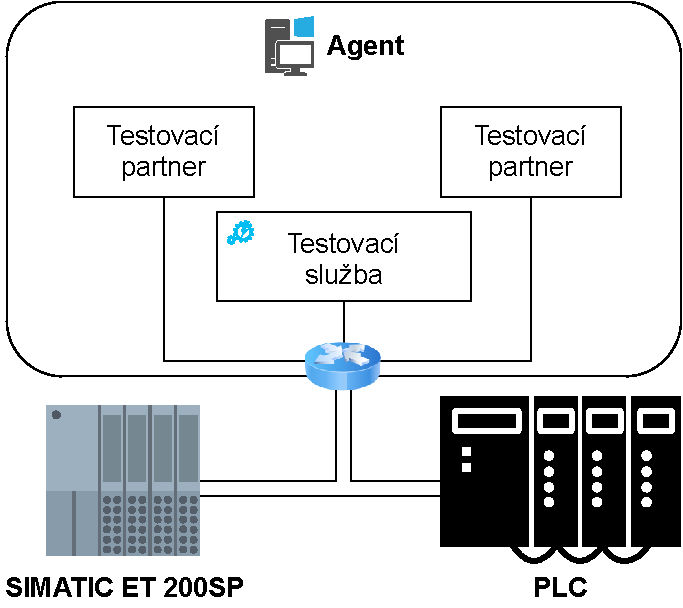
\includegraphics[width=0.97\textwidth]{assets/img/bp_assets/devicemodel.pdf}
    \caption{Ukázka možného propojení účastníků testování v původní knihovně}
    \source{Převzato z \cite{bakalarka}}
    \label{fig:bp_devicemodel}
\end{figure}


\subsection{Integrace do testovaného zařízení}

K tomu aby mohla být knihovna použita na zařízení, které je testováno, je zapotřebí nejdříve implementovat rozhraní pro testované zařízení. Implementací rozhraní jsou definovány primárně všechny potřebné funkce pro vytvoření spojení mezi testovaným zařízením a testovací službou. Zároveň definujeme funkci pro získávání instancí jednotlivých testů. 

Tyto testy rovněž dodržují jednotnou podobu pomocí rozhraní testu. Toto rozhraní definuje tři fáze testu:

\begin{enumerate}
    \item Příprava na testování -- definování potřebných struktur, inicializace.
    \item Testování -- provedení samotného testu.
    \item Úklid po testu -- uvolnění využitých zdrojů a uvedení zařízení do původního stavu.
\end{enumerate}

Všichni účastníci testu musí mít pro provedení daného testu obsahovat implementaci daného testu, definovanou rozhraním pro test, a musí být na základě obdržení identifikátoru testu schopni test instanciovat. To se provede registrací testu ve funkci \inlinecode{getTest}, která je definována rozhraním pro zařízení.

Testovací služba následně synchronizuje všechny účastníky, tak aby před započetím další testovací fáze všechna zařízení dokončila fázi předchozí. 

\subsection{Virtualizační možnosti knihovny}

Testovací knihovna aktuálně nepodporuje virtualizaci, jenž byla definováno v sekci \ref{sec:virtualization}. Všechna zařízení, která byla vytvořena testovací knihovnou běžela na stejném operačním systému bez žádného oddělení.

Testovací knihovna ovšem podporuje tzv. testovací partnery. Tato zařízení slouží k simulaci protistrany při testovaní komunikace s testovaným produktem. Ti byly vytvořeny tak, aby běželi nezávisle od testovací služby na vlastním vlákně. Implementace testovacího partnera pak už pouze požadovala dodání implementace testu, jelikož logika běhu zařízení byla už v testovací knihovně obsažena.

Každý testovací partner má životnost pouze v průběhu testu. To znamená, že před započetím testu je každý testovací partner vytvořen a připojen k testovací službě a následně po dokončení testu ukončen. Toto umožňuje variabilní počet testovacích partnerů pro každý test.

\subsection{Topologie zapojení účastníků testu}

V případě verifikace průmyslové komunikace je samozřejmě podstatné, aby všichni účastníci testu byli schopni komunikovat mezi sebou dle potřeb daných testů. Aktuální knihovna ale toto nijak nekontroluje. 

Jediný požadavek knihovny je, aby každý účastník testu byl připojen k testovací službě a odpovídal na její požadavky. Samotné testované zařízení se připojuje před započetím testování a do konce všech testů musí zůstat připojeno. Testovací partneři, jak už jsem zmínil, se připojují dle potřeby před započetím jednotlivých testů.

Knihovna tedy nijak neřeší topologii zapojení jednotlivých zařízení. Je zde tedy předpoklad, že testovací partneři budou schopni komunikovat s ostatními účastníky testu díky tomu, že samotná testovací služba je schopna s nimi komunikovat. Zároveň, pokud by z nějakého důvodu komunikace nebyla možná, tak musí selhat samotné testy.

\subsection{Souhrn}

I když testovací knihovna přináší zjednodušení a zautomatizovaní testování průmyslové komunikace, stále je zde prostor pro zlepšení. Knihovna v aktuální podobě podporuje pouze limitovanou virtualizaci. Za pomoci knihovny jsme sice schopni simulovat protistranu, ale již ne samotné zařízení a to vždy musí běžet nezávisle na knihovně. 

Aktuální nový požadavek na řešení topologie zapojení zařízení nesplňuje vůbec. Zároveň v již existujícím řešení limitující požadavek, že pro každý test musí každý účastník testu obsahovat implementaci testu. Toto nemusí být vždy potřeba, například při testování veřejného rozhraní. 

\section{Možnosti rozšíření virtualizačních prvků}

Z analýzy stávajícího stavu knihovny je vidět, že možnost virtualizace prostřednictvím stávající knihovny jsou limitované. Knihovna nepodporuje možnost simulovat jakékoliv zařízení a vůbec neřeší topologii zapojení daných zařízení. Rozšířením knihovny tedy chceme docílit větší možnosti simulace jednotlivých zařízení a jejich propojení, čímž se zlepší simulace reálného prostředí. Nová knihovna by tedy měla cílit na

\begin{itemize}
    \item možnost spustit jakékoliv zařízení jako virtualizované,
    \item zapojit tato zařízení dle definované topologie (sériové linky, kruhu, hvězdy).
\end{itemize}

Hlavní motivací je zvýšení flexibility knihovny, rozšíření možností využití a minimalizace úsilí potřebného na testovaní, což vše vede ke snížení nákladů na testování. Tyto kroky také směřují k snížení závislosti na reálném hardwaru, na kterém běží účastníci testů. Je ale samozřejmé, že testy na reálném hardwaru budou vždy potřeba a nelze se této závislosti nijak zbavit.

\subsection{Virtualizace zařízení}

Možností jak virtualizovat zařízení existuje několik. Tyto techniky byly přiblíženy v sekci \ref{sec:virtualization}. Co je tedy nejvhodnějším přístupem k virtualizaci námi požadovaných průmyslových zařízení? 

Jedno z možností je vytvoření VM pro každé virtualizované zařízení. Volba operačního systému poté závisí na zařízení. Pro zachování univerzálnosti hostitelského zařízení dává smysl použití hypervizoru typu II.

Logickou možností je také použití virtualizace skrz kontejnerizaci. Díky kontejnerizaci nemusíme virtualizovat celé operační systémy, ale pouze jejich části, čímž můžeme ušetřit výpočetní zdroje.

Které přístup je tedy efektivnější? Dle studií, které zkoumaly rozdíl ve výkonu a efektivnosti využití výpočetních zdrojů mezi kontejnerizací prostřednictvím softwaru Docker a virtualizačního řešení KVM, který umožňuje jádru fungovat jako hypervizor, vyhrává kontejnerizace. 

Při jejich porovnání bylo zjištěno, že s použitím kontejnerizačního řešení Docker je virtualizovaná zařízení spouštět výrazně rychleji. Tato zařízení také spotřebovávají méně výpočetních zdrojů. V porovnání při počítání HPC(High performance counting) úkolů, bylo dosaženo díky nástroji Docker lepšího výkonu o 42\,\% při úkolech náročných na procesor a o 14,98\,\% lepšího výkonu při úkolech náročných na interní paměť.\cite{kvmdockercomp}\cite{2021virt} 

Jak je tedy vidět, virtualizace kontejnerizací je efektivnější. V následující analýze tedy budeme uvažovat již pouze kontejnerizační řešení. 

\subsection{Porovnání kontejnerizačních řešení}

V dnešní době existuje mnoho řešení, který využívají kontejnerizaci. V následující sekci budou porovnána jednotlivá vybraná řešení a zhodnocena jejich vhodnost pro použití v testovací knihovně. 

Cílem je tedy primárně použít k řešení kontejnerizace tzv. \textit{container engines}. Jejich přímým využitím, oproti využití několika nástrojů, které by dohromady tvořili container engine, doufám předejití problémům s kompatibilitou a integrací těchto nástrojů dohromady.

Hlavním požadavkem na dané řešení je, aby podporovalo operační systém Windows. Tento požadavek primárně vyvstává z infrastruktury firmy Siemens. Vybranými řešeními tedy jsou

\begin{itemize}
    \item Docker,
    \item Podman.
\end{itemize}

Obě tato řešení jsou velice srovnatelná. Jak bylo zmíněno, ve spoustě případů je možné zaměnit příkaz \inlinecode{docker} za \inlinecode{podman} bez žádných problémů. 

Pokud se ovšem zaměříme na jejich rozdíly, tak Docker v základu podporuje více síťových ovladačů. Je ovšem možné také implementovat vlastní síťový ovladač. \cite{docker_networking_overview}

Největší výhoda ovšem nastává v rozšířenosti softwaru Docker. Při pohledu na dostupnost knihoven integrujících software Docker do prostředí .NET, ve kterém běží stávající knihovna, je vidět rovnou několik možností, které lze využít. Oproti tomu pro software Podman tyto integrace neexistují. Při jeho integraci by tedy bylo potřeba vytvořit vlastní integraci. 

Zároveň Podman je navrhnut primárně pro operační systém Linux. Jeho použití je sice na operačním systému možné, ale každý kontejner musí obsahovat hostující Linuxový systém. 

Jak je tedy vidět, pro použití v testovací knihovně je vhodnější využití softwaru Docker. V aktuální podobě jeho použití přináší jasné benefity. 


\section{Možnost propojení s reálnými zařízeními}

Testovací knihovna ve své aktuální podobě podporuje propojení s reálnými zařízeními, na kterých běží implementace propojení s testovací službou. Propojení mezi zařízeními samotnými je teoreticky také možné, ovšem už není nijak kontrolováno či orchestrováno za pomoci testovací knihovny. 

Vyvstává zde tedy otázka, zdali je teoreticky možné propojit jednotlivá virtualizovaná zařízení s reálnými zařízeními, která běží mimo zařízení, na kterém běží virtualizované prostředí. K tomu aby bylo možné toto analyzovat, předpokládejme dále využití softwaru Docker pro virtualizaci v testovací knihovně.

\subsection{Analýza}

Jednotlivé Docker kontejnery nemají ponětí o propojení s externí sítí, tedy sítí, mimo virtualizované prostředí. Kontejnery, pokud jsou připojeny k nějaké síti, mají pouze znalost o implicitní bráně, na kterou směrují všechnu komunikaci. Pokud kontejnery nejsou izolované, tak jsou takto schopné dosáhnout hostujícího stroje a tím i externí sítě. V komunikaci ve směru od virtualizovaného zařízení k reálnému zařízení by tedy neměl být problém. \cite{docker_brige_overview}

Problém může ovšem nastav v opačném směru. Jednotlivé kontejnery v základním nastavení nejsou dostupné z externí sítě. Docker ovšem podporuje přesměrování portů. Tímto způsobem je možné namapovat port z virtualizovaného prostředí na port na hostujícím zařízení, na který je následně směřováno komunikace z externího zařízení. \cite{docker_ports}

Vyvstává zde ale problém vznikající primárně z definice jednotlivých komunikačních protokolů. Tyto protokoly často běží na specifickém portu a tedy komunikace s více než jedním zařízením může způsobit kolizi těchto portů. To může zapříčinit neschopnost komunikace se všemi virtualizovanými zařízeními. 

\subsection{Shrnutí}

Jak z analýzy vyplívá, komunikace s reálnými zařízení je teoreticky možná. Ze specifika daného problému a protokolů využitých ke komunikaci ovšem nelze nyní komunikovat s externími zařízeními. K tomu aby byla komunikace možná, tak je potřeba nejdříve vyřešit problém kolize portů, pokud tedy nějaké řešení pro tento problém existuje. 

